\documentclass{sintefbeamer}

% packages, font, color, and newcommands
\usepackage{amsfonts, amsmath, oldgerm, lmodern, bm}
% \usepackage[font={footnotesize}]{caption}
\usepackage{natbib}
\usepackage{url}
\usepackage{tikz}
\usepackage{amssymb}
\usepackage{amsmath}
\usepackage{amsthm}
\usepackage{mathrsfs}
\usepackage{empheq}
\usepackage{mdframed}
\usepackage{bm}
\usepackage{animate}
\usepackage{xcolor,colortbl}
\usepackage{graphicx}
\bibliographystyle{apalike}
\usefonttheme{serif}
\usetikzlibrary{calc}

\title{A phenomenological description of pairwise interactions in buoyant driven emulsions.}
\subtitle{based on the nearest pair statistic}
\author{\href{http://basilisk.fr/sandbox/fintzin/Rising-Suspenion/RS.c}{\underline{N. Fintzi}\footnote{IFP \'Energies Nouvelles, France}$^{,2}$}, JL. Pierson$^1$ and S. Popinet\footnote{Sorbonne Universit\'e, France}}
% \date{Created on May 22, 2022}

\titlebackground{image/3D/P_PHI_5.png}

% document body
\addtobeamertemplate{navigation symbols}{}{%
    \usebeamerfont{footline}%
    \usebeamercolor[fg]{footline}%
    % \hspace{1em}%
    % \vspace{1em}%
    \insertframenumber/\inserttotalframenumber
}
\usepackage{stmaryrd}
\newcommand{\Jump}[1]{\llbracket #1 \rrbracket \cdot \textbf{n} }

\newcommand{\size}{0.22\textwidth}
\newcommand{\avg}[1]{\left<#1\right>}
%\newcommand{\condavg}[1]{\left<#1 | \mathscr{C}_1\right>}
\newcommand{\Exp}[1]{\overline{\overline{#1}}}
\newcommand{\davg}[1]{\left<#1\right>_d}
\newcommand{\avgcond}[1]{\overline{#1}}
% \renewcommand{\avgcond}[1]{\left{#1}}
\newcommand{\kavg}[1]{\avgcond{#1}^k}
\newcommand{\cavg}[1]{\avgcond{#1}^c}
\newcommand{\Tavg}[1]{\avgcond{#1}^T}
\newcommand{\Xavg}[1]{\avgcond{#1}^X}
\newcommand{\TXavg}[1]{\Tavg{\Xavg{#1}}}
\newcommand{\Iavg}[1]{\left<#1\right>_I}
\newcommand{\pavg}[1]{n \left<#1\right>}
\newcommand{\pnavg}[1]{\left<#1\right>}
\newcommand{\nstavg}[1]{\overline{#1}^{nst}}
\newcommand{\condavg}[2]{\overline{#1}^{#2}}
\newcommand{\nstrelavg}[1]{\overline{#1}_{nst}^{rel}}
\newcommand{\mavg}[1]{\left<#1\right>_m}
\newcommand{\gavg}[2][\gamma]{\left<#2\right>_{#1}}
\newcommand{\partials}[1]{\partial_{i_1}\partial_{i_2}\ldots\partial{i_{#1}}}
\newcommand{\partialp}[2]{ \prod_{m=#1}^{#2} \partial_{i_m}}
\newcommand{\hatpartialp}[2]{ \prod_{m=#1}^{#2} \hat{\partial}_{j_m}}
\newcommand{\hatpartialpi}[2]{ \prod_{m=#1}^{#2} \hat{\partial}_{i_m}}
\newcommand{\pri}[2]{ \prod_{m=#1}^{#2} r_{i_m}}
\newcommand{\prj}[2]{ \prod_{m=#1}^{#2} r_{j_m}}
\newcommand{\nablab}{\bm{\nabla}}
\newcommand{\nablabh}{\hat{\bm{\nabla}}}
\newcommand{\ddt}{\frac{d}{d t}}
\newcommand{\pddt}{\partial_t}
% \newcommand{\pddt}{\partial t \;}

\newcommand{\CC}{\mathscr{C}}
\newcommand{\tb}[1]{\color{blue}#1\color{black}}
% \renewcommand{\tb}[1]{}

% \renewcommand{\ref}[1]{\autoref{#1}}
\renewcommand{\size}[1]{0.3\textwidth}
\newcommand{\expo}[1]{\frac{(-1)^n}{n!} \partialp{1}{n} \pavg{\int_{\Omega_\alpha} \pri{1}{n}#1 d\Omega}}

\usepackage{amsmath}

\logo{\includegraphics[height=1cm]{overleaf-logo}}


\begin{document}
% \maketitle

% \begin{frame}
%   \frametitle{Industrial context}
%   \underline{Coalescence is ubiquitous in chemical engineering processes :}
%   \begin{itemize}
%     \item Separation processes (gravity separators, flotation)
%     \item Bubble column reactors
%     \item Liquid-liquid separation
%   \end{itemize}
%   \vfill
%   \underline{In all those process we need to : }
%   \begin{itemize}
%     \item Predict global hydrodynamics in disperse bubbly flows and emulsion (interphase drag forces \ldots).
%     \begin{itemize}
%       \item Model of coalesce and size distribution 
%       \begin{itemize}
%         \item Understand the interactions between pairs of droplets
%       \end{itemize}
%     \end{itemize}
%   \end{itemize}

%   \vfill
%   Therefore, in this work focuses on the study of \textbf{pair interactions} in oil/water \textbf{emulsions}.
% \end{frame}


% \begin{frame}{Multiscale problem : 1. Solve, 2. Needs and 3. Provides}
  
% 	\textbf{Reactor scale or Macroscale :} 
%     \hfill\underline{PhD R17, Kamel Landal}
%     \begin{enumerate}
%       \item Averaged Navier-Stokes and Population Balance Equations. 
%       \item Drag forces, velocity fluctuation and \textbf{coalescence kernel} closure terms. 
%       \item Optimize industrial processes. 
%     \end{enumerate}

%     \textbf{Drop-scale or Microscale : } 
%     \hfill\underline{PhD R17, Nicolas Fintzi}
%     \begin{enumerate}
%       \item Navier-Stokes two-phase flows equations. 
%       \item Film drainage time.  
%       \item \textcolor{blue}{Closure for \textbf{Macro-scale}, (interphase drag forces, velocity fluctuations \ldots) And \textcolor{red}{pairs interactions modeling} for the \textbf{Nano-scale}  problem.}  
%     \end{enumerate}

%     \textbf{Film-scale or Nanoscale :}
%     \hfill\underline{Future PhD R17 2024}
% 	\begin{enumerate}
% 		\item Film drainage equations. 
% 		\item Interaction models microscale hydrodynamic.   
% 		\item Time of coalescence closure.  
% 	\end{enumerate}
%   \centering
%   \begin{tikzpicture}[very thick]
%     \node[draw] (macro) at (-2,0){Macroscale};
%     \node[draw] (micro) at (4,0){Microscale};
%     \node[draw] (nano) at (8,0){Nanoscale};
%     \draw[<-,blue](macro) -- (micro);
%     \node[draw,dashed] (meso) at (1,0.5){Mesoscale};
%     \draw[dashed,->,blue](micro) -- (meso.east);
%     \draw[dashed,<-](macro) -- (meso.west);
%     \draw[->,red](micro) to[bend left] (nano);
%     \draw[->](nano) to[bend left] (micro);
% \end{tikzpicture}
% \end{frame}

\section{Theoretical modeling of mesoscale equations to describe relative interactions}
\section*{}

\begin{frame}{General form of the kinetic theory.}
  \begin{definition}
    \begin{itemize}
      \item Let $\mathscr{C} =\left\{\textbf{x}_1,\textbf{u}_1, \textbf{q}_1\ldots\textbf{x}_N,\textbf{u}_N, \textbf{q}_N\right\}$ be the vector containing all the particles' internal coordinates such as their velocities and positions vectors and any other arbitrary particles' quantities $\textbf{q}$. 
      \item Then $P(\mathscr{C},t)$ is the probability density function of finding the flow in the state $\mathscr{C}$, at time $t$. 
    \end{itemize}
  \end{definition}
  Transport equation of the Probability Density Function (PDF) is defined as,
  \begin{equation}
    \pddt P(\mathscr{C},t)
    + \frac{\partial}{\partial \mathscr{C}} \cdot
    \left[
        \frac{d\mathscr{C}}{dt}  
        P(\mathscr{C},t)
    \right]
    = \Psi(\mathscr{C})
    \label{eq:dt_P}
\end{equation}

  \begin{itemize}
    \item $\Psi(\mathscr{C})$ is the source term due to the particles' interactions, such as break-up coalesce and collisions phenomenons. 
  \end{itemize}
  \begin{equation*}
    \Psi(\mathscr{C}) =
    \underbrace{B(\mathscr{C})}_{\text{Break-up}}
    +\underbrace{S(\mathscr{C})}_{\text{Coalescence}}
  \end{equation*}
\end{frame}

\begin{frame}{The point PDF for Population Balance Equations.}
  \begin{definition}
    \begin{itemize}
      \item Let $\mathscr{C} =\left\{\textbf{x}_1,\textbf{u}_1,d_1\right\}$ be the vector containing a  particles' velocity, position vectors and diameters. 
      \item Then $P_1(\textbf{x},\textbf{u},d,t)$ is the probability density function of finding this particle at the position $\textbf{x} = \textbf{x}_1$, $d = d_1$ and $\textbf{u} = \textbf{u}_1$.  
    \end{itemize}
  \end{definition}
  Transport equation of the one point PDF reads as,
  \begin{equation}
    \pddt P_1
    + \partial_{\textbf{x}} \cdot
    (\textbf{u}P_1)
    + \partial_{\textbf{u}} \cdot
    (\textbf{f}P_1)
    + \partial_{d} \cdot
    (\dot{d} P_1)
    = \Psi(\textbf{x},\textbf{u},d,t)
    \label{eq:dt_P_1}
\end{equation}

  \begin{itemize}
    \item $\textbf{f} = \ddt \textbf{u}$ is the forces per unit of mass applied on the particle test. 
    \item By Multiplying Eq. (\ref{eq:dt_P_1}) by the momentum or the mass and integrating on all \textbf{u} we would recover the conservation equation for respectively the momentum or the mass. 
  \end{itemize}
\end{frame}


\begin{frame}{The nearest particle PDF to derive relative interactions equations (DZ Zhang, PoF, 2023)}
  \begin{definition}
    \begin{itemize}
      \item Let $\mathscr{C} =\left\{\textbf{x}_1, \textbf{r}, \textbf{w},a\right\}$ be the vector containing the position of a particle $\textbf{x}_1$, its nearest neighboring particle relative position $\textbf{r}$, the relative velocity \textbf{w} and the age of the pair time interaction $a$.
      \item Then, $P_{nst}(\textbf{x},\textbf{r},\textbf{w},a) $ is the probability of finding a particle at \textbf{x} with its nearest neighboring particle at \textbf{r} with a relative velocity of \textbf{w}. 
    \end{itemize}
  \end{definition}
  Transport equation of the reduced PDF,
  \begin{equation*}
    \underbrace{
      \pddt P_{nst}
      +  \partial_{\textbf{x}} \cdot
      \left(
        \nstavg{\textbf{u}}
        P_{nst}
      \right)
      % +  \partial_{textbf{u}} \cdot
      % \left(
      %   \nstavg{\textbf{a}}
      %   P_{nst}
      % \right)
    }_{\text{Macroscopic scale}}
    + 
    \underbrace{
       \partial_a 
        P_{nst}
      + \partial_{\textbf{r}} \cdot
    \left(
        \nstavg{\textbf{w}}
        P_{nst}
    \right)
      +  \partial_{\textbf{w}} \cdot
    \left(
        \nstavg{\textbf{a}}
        P_{nst}
    \right)
    }_{\text{inter-particle scale}}
    = \Psi
    \label{eq:dt_P_nst}
\end{equation*}

  \begin{itemize}
    \item $\nstavg{\textbf{u}}(\textbf{x},\textbf{r}) = \ddt \textbf{x}_1$ is the particle velocity at \textbf{x} knowing a particle at \textbf{r}. 
    \item $\nstavg{\textbf{w}}(\textbf{x},\textbf{r}) = \ddt \textbf{r}$ is the nearest particle \textbf{relative} velocity. 
    \item $\nstavg{\textbf{a}}(\textbf{x},\textbf{r}) = \ddt \textbf{w}$ is the averaged relative acceleration.
  \end{itemize}
  \underline{In this work we will be interested in the \textbf{nearest particle statistic} $P_{nst}$}
\end{frame}


\section{Numerical investigation of drops interactions}

\section*{}
\begin{frame}
\frametitle{Direct Numerical Simulation of buoyant emulsions}
\begin{columns}
  \column{0.6\textwidth}
\underline{Simulation set up :} 
\begin{itemize}
  \item Tri -periodic boundary conditions. 
  \item Mono-disperse distribution of droplets size.
  \item We prevent coalesce by the use of a special algorithm 
  (\href{http://basilisk.fr/sandbox/fintzin/Rising-Suspension/no-coalescence.h}{no-coalescence.h})
  \item Free software : \url{https://basilisk.fr}
\end{itemize}

\begin{figure}
  \caption{Snapshot of a simulation at $T_g = 300$ for $\phi = 0.01$, $Ga = 75$ $\mu_r = 0.1$ and $N_b = 125$. In white : the interfaces, The background color map correspond to the pressure field. The grid represents the different core ($\le 729$ !).
  }
\end{figure}
\column{0.5\textwidth}
\centering
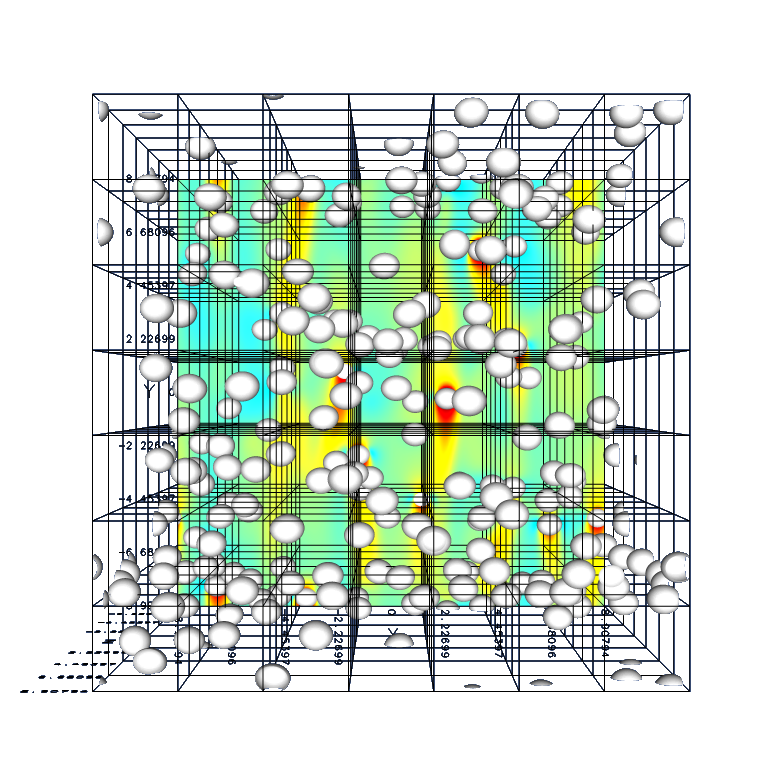
\includegraphics[width =  1.1\textwidth]{image/PHI_01_Ga_75.png}
\end{columns}
\end{frame}

\begin{frame}
  \frametitle{Direct Numerical Simulation of buoyant emulsions}
  \begin{columns}
    \column{0.6\textwidth}
  \underline{Dimensionless parameters :} 
  \begin{itemize}
    \item \textit{Galileo} number : $Ga =\frac{\sqrt{\rho \Delta\rho gD^3}}{\mu} \in [5, 100]$
    \item \textit{Bond} number : $Bo = \frac{\Delta \rho g D^2}{\sigma} = 1$ 
    \item volume fraction of dispersed phase : $\phi = [0.01;0.15]$. 
    \item Density and viscosity ratio, $\rho_r=1.11$ and $\mu_r= 0.1$. 
  \end{itemize}
  
  \begin{figure}
    \caption{Snapshot of a simulation at $T_g = 300$ for $\phi = 0.01$, $Ga = 75$ $\mu_r = 0.1$ and $N_b = 125$. In white : the interfaces, The background color map correspond to the pressure field. The grid represents the different core ($\le 729$ !).
    }
  \end{figure}
  \column{0.5\textwidth}
  \centering
  \href{file:///work/fintzin/BUBLLES_PROJECT/movies/cut.gif}{\beamergotobutton{Play}}
  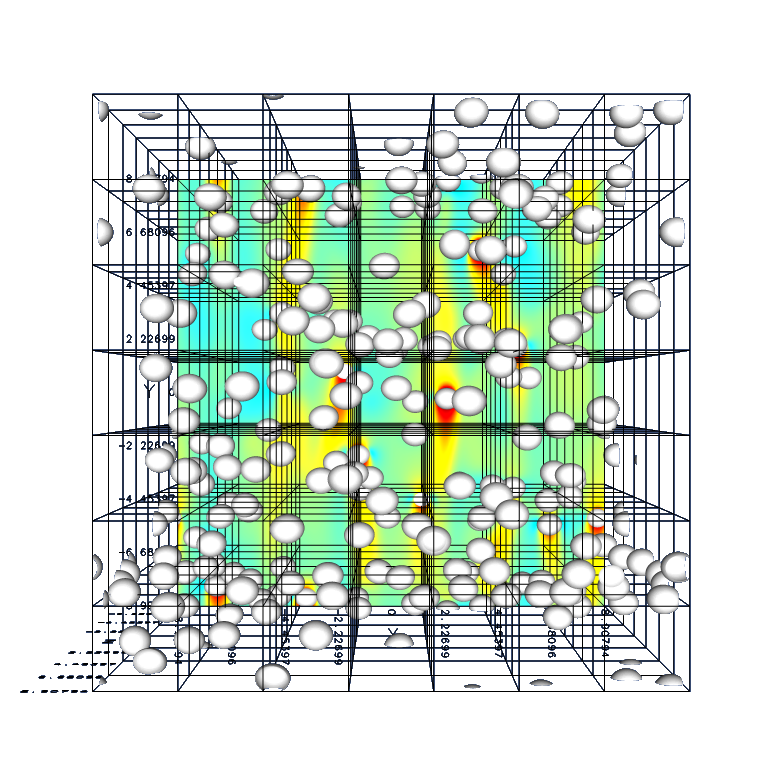
\includegraphics[width =  1.1\textwidth]{image/PHI_01_Ga_75.png}
  \end{columns}
\end{frame}

\begin{frame}
  \frametitle{Nearest pair probability density function}

  \begin{columns}
    \column{0.7\textwidth}
    \centering
    \begin{tabular}{cccc}
      &
      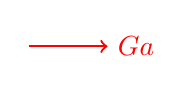
\begin{tikzpicture}[color=red]
        \draw[thick,->] (0,0) -- (1,0)node[right]{$Ga$};
      \end{tikzpicture}& & \\ 
        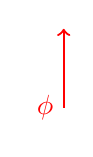
\begin{tikzpicture}[color=red]
          \draw[thick,<-] (0,0) -- (0,-1)node[left]{$\phi$};
        \end{tikzpicture} 
        &
        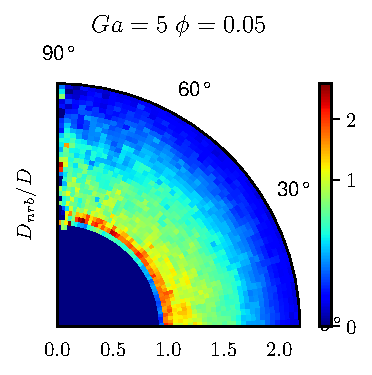
\includegraphics[height=0.3\textwidth]{image/HOMOGENEOUS/fDrop/Pnst_mu_r_1_0_Ga_5_PHI_0_05.pdf}  &
        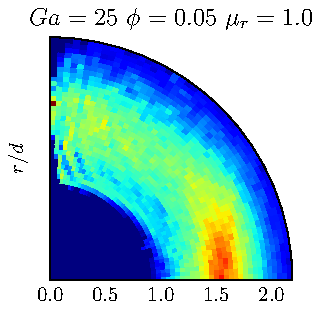
\includegraphics[height=0.3\textwidth]{image/HOMOGENEOUS/fDrop/Pnst_mu_r_1_0_Ga_25_PHI_0_05.pdf} &
        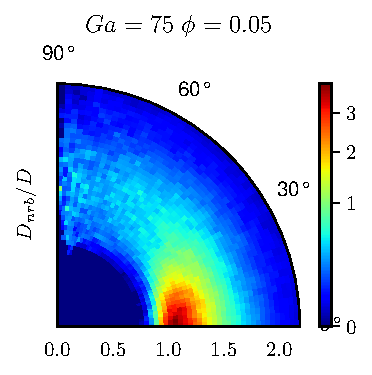
\includegraphics[height=0.3\textwidth]{image/HOMOGENEOUS/fDrop/Pnst_mu_r_1_0_Ga_75_PHI_0_05.pdf} 
        \\
         &
          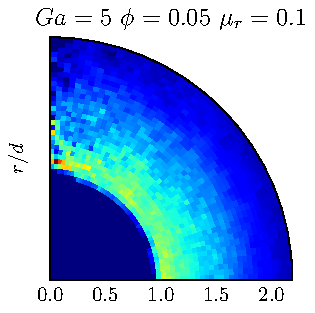
\includegraphics[height=0.3\textwidth]{image/HOMOGENEOUS/fDrop/Pnst_mu_r_0_1_Ga_5_PHI_0_05.pdf} &
        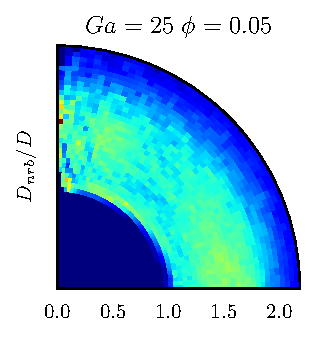
\includegraphics[height=0.3\textwidth]{image/HOMOGENEOUS/fDrop/Pnst_mu_r_0_1_Ga_25_PHI_0_05.pdf}&
        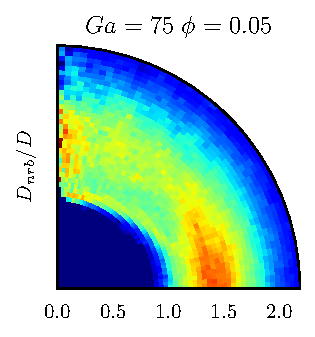
\includegraphics[height=0.3\textwidth]{image/HOMOGENEOUS/fDrop/Pnst_mu_r_0_1_Ga_75_PHI_0_05.pdf}\\
      \end{tabular}

      \column{0.3\textwidth}
      \begin{figure}
        \caption{Plots of $P_{nst} (\textbf{r})$ for different $Ga$ and $\phi$.}
      \end{figure}
    
    \begin{itemize}
      \item Drafting -Kissing tumbling mechanism for low $\phi$ and high $Ga$. 
    \end{itemize}
  \end{columns}
\end{frame}

\begin{frame}
  \frametitle{Reconstruction of the nearest relative velocity fields}

  \begin{figure}
    
    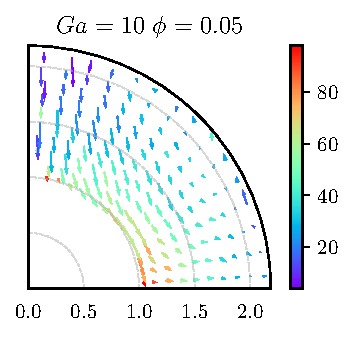
\includegraphics[height=0.25\textwidth]{image/HOMOGENEOUS/fDrop/U_mu_r_0_1_Ga_10_PHI_0_05.pdf}
    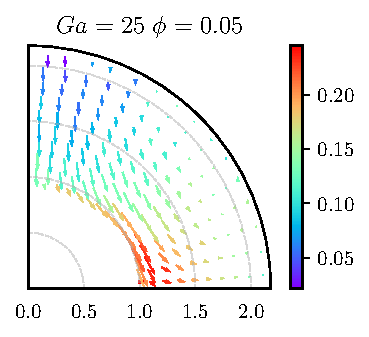
\includegraphics[height=0.25\textwidth]{image/HOMOGENEOUS/fDrop/U_mu_r_0_1_Ga_25_PHI_0_05.pdf}
    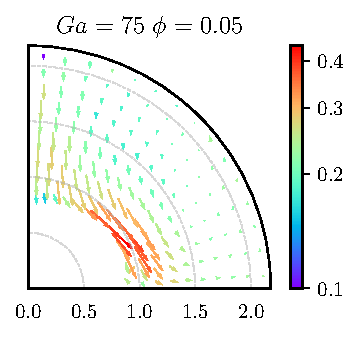
\includegraphics[height=0.25\textwidth]{image/HOMOGENEOUS/fDrop/U_mu_r_0_1_Ga_75_PHI_0_05.pdf}
    
    \caption{Nearest averaged velocity fields, $\nstavg{\textbf{w}} (\textbf{r},a)$ for different $Ga$ and $\phi$. 
    Colormap : dimensionless age of interaction $a$. }
  \end{figure}

\begin{itemize}
  \item In average particles approach from the top and leave through the sides. 
  % \item How to quantify this phenomenon ? 
  \item Representation of the Drafting -Kissing tumbling mechanism since the velocity fields converge toward high density zone. 
\end{itemize}
$\rightarrow$ How to quantify these fields ?
\end{frame}

\begin{frame}
  \frametitle{Computation of the correlation tensor $\mathbb{S}$ }
  \begin{figure}
    \begin{centering}
      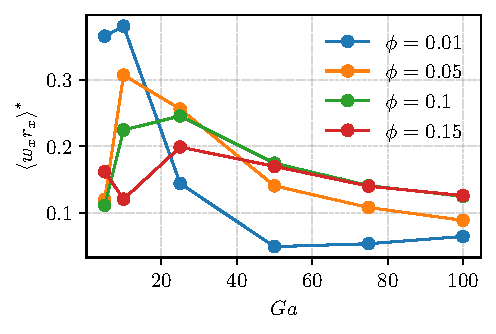
\includegraphics[height=0.25\textwidth]{image/HOMOGENEOUS/fPA/URxx.pdf}
      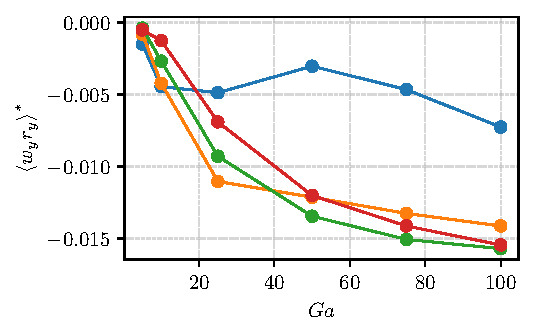
\includegraphics[height=0.25\textwidth]{image/HOMOGENEOUS/fPA/URyy.pdf}
      % 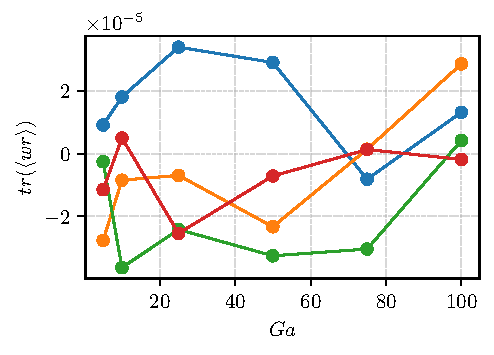
\includegraphics[height=0.2\textwidth]{image/HOMOGENEOUS/fPA/UR.pdf}
      \caption{Dimensionless correlation tensor $\mathbb{S} =  \int \textbf{r}\nstavg{\textbf{w}} P_{nst}(\textbf{x},\textbf{r})d\textbf{r}$}
    \end{centering}
  \end{figure}

  \begin{itemize}
    \item $\mathbb{S}_{xx} = \int r_x\nstrelavg{u_x} > 0$ \textbf{outward} particle flux.  
    \item $\mathbb{S}_{yy} = \int r_y\nstrelavg{u_y} < 0$ \textbf{inward} particle flux. 
    \item $\text{tr}\left(\mathbb{S}\right) = 0$ conservation of the number of the nearest particle flux. 
  \end{itemize} 
\end{frame}


\begin{frame}{The averaged nearest relative velocity equation}
  \begin{equation}
      \pddt P_{nst}
      +  \partial_{\textbf{x}} \cdot
      \left(
        \nstavg{\textbf{u}}
        P_{nst}
      \right)
      % +  \partial_{textbf{u}} \cdot
      % \left(
      %   \nstavg{\textbf{a}}
      %   P_{nst}
      % \right)
    + 
       \partial_{\textbf{r}} \cdot
    \left(
        \nstavg{\textbf{w}}
        P_{nst}
    \right)
    = \Psi
    \label{eq:dt_P_nst1}
\end{equation}
Multiplying Eq. (\ref{eq:dt_P_nst1}) by \textbf{rr}, yields :
%  the \textbf{Mean square particles distance conservation equation  :}
\begin{equation*}
  \pddt \mathbb{R} 
+ \partial_{\textbf{x}} \cdot (\mathbb{R} \condavg{\textbf{u}_i}{1}
% + \avg{\delta_i\textbf{u}_i' (\textbf{r} \textbf{r})'}
)
= 
 \mathbb{S}
+ \avg{\textbf{r}\textbf{r}\Psi}
\end{equation*}

\begin{itemize}
  \item $\mathbb{R} = \int \textbf{rr} P_{nst} d\textbf{r}$ Mean square distance to the nearest particle. 
  \item $\mathbb{S} = \int \textbf{r} \nstavg{\textbf{w}}P_{nst} d\textbf{r}$ is the  correlation between $\nstavg{\textbf{w}}$ and $\textbf{r}$. 
  % \item $\int \textbf{rr} \dot{P_{nst}} d\textbf{r}$  source term tensor, still accounting for coalesces and breakup. 
\end{itemize}

$\rightarrow$ Consequently, the tensor $\mathbb{R}$ is plan isotropic due to the form of $\mathbb{S}$.

$\rightarrow $ $\mathbb{R}$ is the mathematical representation of the mesoscale structures (cluster \ldots)
\vfill
\begin{figure}
  \centering
  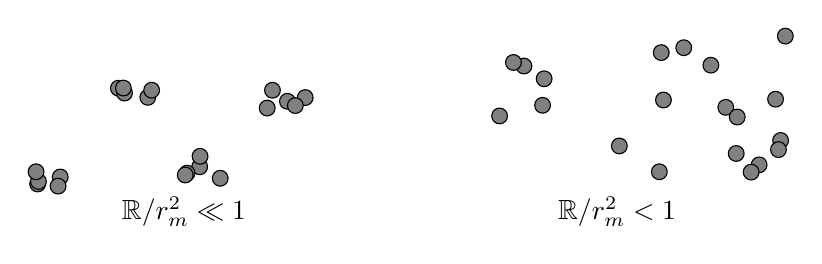
\begin{tikzpicture}
    
  \foreach \i in {1,...,5} {
  \pgfmathsetmacro{\x}{rnd*0.7}
  \pgfmathsetmacro{\y}{rnd*0.3}
  \draw[fill=gray] ($(\x,\y)$) circle (0.1);
  }
  \foreach \i in {1,...,5} {
  \pgfmathsetmacro{\x}{rnd*0.7}
  \pgfmathsetmacro{\y}{rnd*0.3}
  \draw[fill=gray] ($(\x+2,\y)$) circle (0.1);
  }
  \foreach \i in {1,...,5} {
  \pgfmathsetmacro{\x}{rnd*0.6}
  \pgfmathsetmacro{\y}{rnd*0.4}
  \draw[fill=gray] ($(\x+1,\y-1)$) circle (0.1);
  }
  \foreach \i in {1,...,5} {
  \pgfmathsetmacro{\x}{rnd*0.6}
  \pgfmathsetmacro{\y}{rnd*0.4}
  \draw[fill=gray] ($(\x-1,\y-1)$) circle (0.1);
  }
  \draw (1,-1)node[below]{$\mathbb{R}/r_m^2 \ll 1$};

    \foreach \i in {1,...,20} {
      \pgfmathsetmacro{\x}{rnd*4}
      \pgfmathsetmacro{\y}{rnd*2}
      \draw[fill=gray] ($(\x+5,\y-1)$) circle (0.1);
      }
      \draw (6.5,-1)node[below]{$\mathbb{R}/r_m^2 < 1$};
    \end{tikzpicture}
    \hfill
\end{figure}


\end{frame}



\begin{frame}
  \frametitle{Representation of the interaction force}

  \begin{figure}
    % 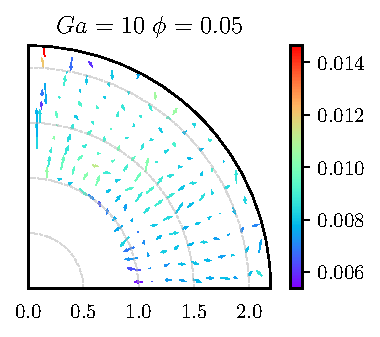
\includegraphics[height=0.25\textwidth]{image/HOMOGENEOUS/fDrop/F_mu_r_0_1_Ga_10_PHI_0_05.pdf}
    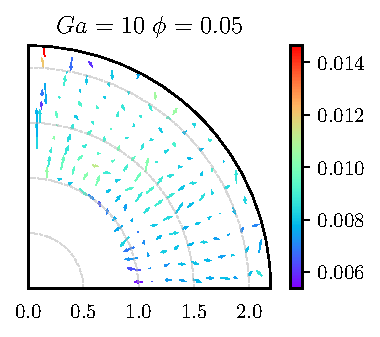
\includegraphics[height=0.25\textwidth]{image/HOMOGENEOUS/fDrop/F_mu_r_0_1_Ga_10_PHI_0_05.pdf}
    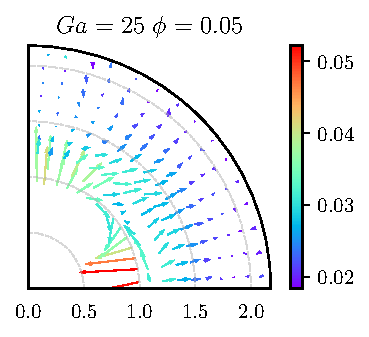
\includegraphics[height=0.25\textwidth]{image/HOMOGENEOUS/fDrop/F_mu_r_0_1_Ga_25_PHI_0_05.pdf}
    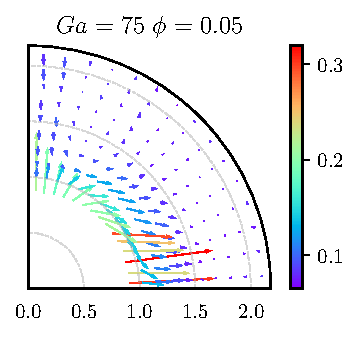
\includegraphics[height=0.25\textwidth]{image/HOMOGENEOUS/fDrop/F_mu_r_0_1_Ga_75_PHI_0_05.pdf}
    
    \caption{Nearest averaged relative acceleration fields times the mass of a particle $\nstavg{\textbf{f}}(\textbf{r},a)$. 
    Color map : Dimensionless age of the interaction.}
  \end{figure}

  
\begin{itemize}
  % \item $\nstrelavg{\textbf{F}}$ is an isotropic repulsion force at high $Ga$. 
  % \item At lower $Ga$ we observe attraction forces $\nstrelavg{\textbf{F}}$ on the sides.
  \item The force is always repulsive on the vertical direction.  
  \item On the sides  directions, Long time interactions results into attraction forces, while short time interaction into repulsion forces.
  \item Attraction forces might lead to coalesence. 
\end{itemize}

$\rightarrow$ How to quantify these fields ? 
\end{frame}




\begin{frame}{The averaged nearest relative momentum equation}
  
  Multiplying the transport equation of $P_{nst}$ by \textbf{rw}, yields, 
  % and integrating  over  all  \textbf{r} and \textbf{w} yields the \textbf{Mean relative momentum correlation equation :}
  
  \begin{equation*}
    \pddt \mathbb{S} 
  + \partial_{\textbf{x}} \cdot (
    \condavg{\textbf{u}}{1} 
    \mathbb{S})
  % + P_1\condavg{\textbf{u}_i' (\textbf{r}\textbf{w}_{ij})'}{1})
  = \avg{\textbf{w}\textbf{w}}
  + \Sigma_{B}
  + \Sigma_{PFP}
  + \avg{\textbf{w}\textbf{r}\Psi}
\end{equation*}
  
  \begin{itemize}
      \item Fluctuation of the velocity $\avg{\textbf{w}\textbf{w}} \approx \avg{\textbf{u}_i'\textbf{u}_i'}$ (related to the Reynolds stress)
    \item $\mathbf{\Sigma}_{PFP} = \int \textbf{r} \nstavg{\textbf{F}} P_{nst} d\textbf{r}d\textbf{w}$ correlation between \textbf{r} and the hydrodynamic  drag force on the particle $\nstavg{\textbf{F}}$\footnote{(DZ Zhang, JFM, 2021 : \textbf{particle fluid particle stress})}. 
    \item $\mathbf{\Sigma}_{B} = \int \textbf{r} \nstrelavg{\textbf{b}} P_{nst} d\textbf{r}d\textbf{w} = 0$, correlation between \textbf{r} and the \textbf{relative body} forces applied on the pair of nearest particles.
  \end{itemize}
  
  $\rightarrow$  The relative motion between particles are driven by $\avg{\textbf{w}\textbf{w}}$ and $\Sigma_{PFP}$.
  
  \end{frame}
  

\begin{frame}
  \frametitle{Computation of the Particle Fluid Particle (PFP) stress}
  \underline{What is the particle stress (Zhang, JFM, 2021) ?}  
   : $\avg{\text{Drag Force}} = \avg{F} + \nablab \cdot \Sigma_{PFP}$
  \begin{figure}
    % 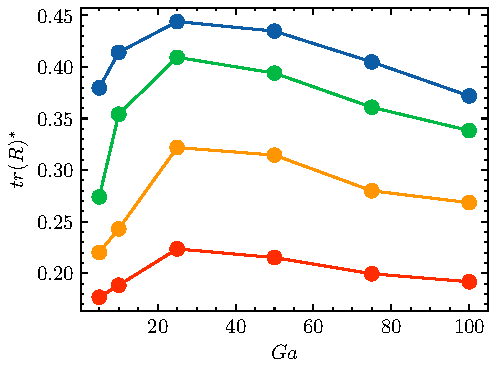
\includegraphics[height=0.23\textwidth]{image/HOMOGENEOUS/fPA/RR.pdf}
    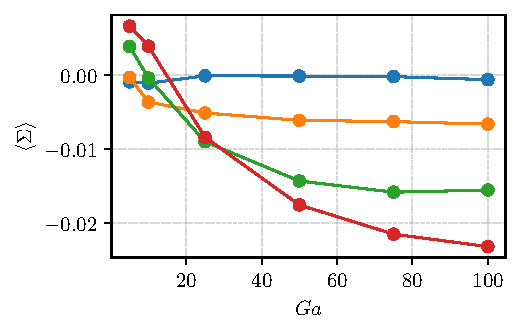
\includegraphics[height=0.23\textwidth]{image/HOMOGENEOUS/fPA/PFP.pdf}
    \caption{ 
      % (left) Dimensionless  mean square distance to the nearest neighbor ($\textbf{R}^* =0$ particle in contact). 
      (right) Particle fluid particle stress $\mathbf{\Sigma}_{PFP} = \int \textbf{r}\nstavg{\textbf{f}} P_{nst}d\textbf{r}$.
      }
  \end{figure}
  
\begin{itemize}
  \item $\text{tr}(\mathbf{\Sigma}_{PFP}) > 0$ global repulsion for high $\phi$ and $Ga$. 
  \item $\text{tr}(\mathbf{\Sigma}_{PFP}) < 0$ global attraction for small $Ga$ and $\phi$.
  % \item $\text{tr}(\mathbf{\Sigma}_{PFP}) = 0$ no pressure, when $\phi \rightarrow 0$ and $Ga \rightarrow 0$. 
  \item  $\mathbf{\Sigma}_{PFP}$ is then correlated with the mean nearest particle distance $\mathbb{R}$. 
\end{itemize}

\end{frame}
\begin{frame}
  \frametitle{Computation of $\avg{\textbf{ww}}$}
  \begin{figure}
    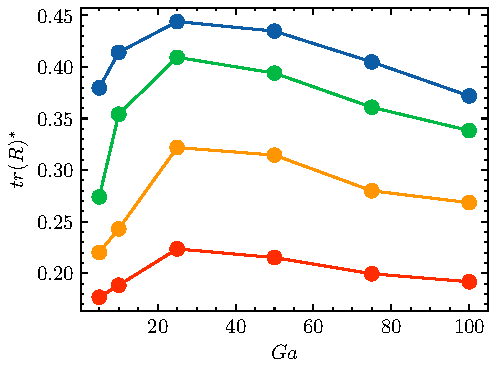
\includegraphics[height=0.23\textwidth]{image/HOMOGENEOUS/fPA/RR.pdf}
    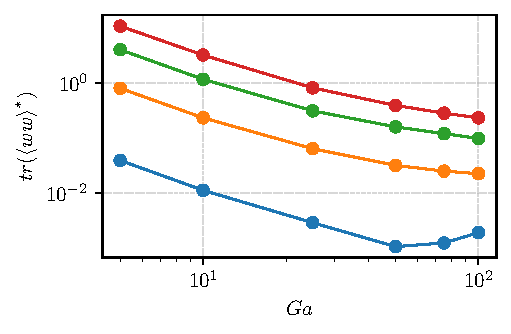
\includegraphics[height=0.23\textwidth]{image/HOMOGENEOUS/fPA/trWW.pdf}
    \caption{ 
      (left) Dimensionless  mean square distance to the nearest neighbor ($\textbf{R}^* =0$ particle in contact). 
      (right) Relative velocity correlation  $\avg{\textbf{ww}}$.
      }
  \end{figure}
  \begin{equation*}
    \frac{D^2 \mathbb{R}}{Dt^2}
  %   \pddt \mathbb{S} 
  % + \partial_{\textbf{x}} \cdot (
  %   \condavg{\textbf{u}}{1} 
  %   \mathbb{S})
  % + P_1\condavg{\textbf{u}_i' (\textbf{r}\textbf{w}_{ij})'}{1})
  = \avg{\textbf{w}\textbf{w}}
  + \Sigma_{PFP}
  + \avg{\textbf{w}\textbf{r}\Psi}
\end{equation*}
  
  
\begin{itemize}
  \item At low inertia the particle come closer because $\Sigma_{PFP}<0$, at high inertia because $\avg{\textbf{ww}} \searrow$
  \item At $Ga \approx 25$ we have the most distant situation. 
\end{itemize}

\end{frame}




% \section{First glimpse of coalescence modeling}
% \section*{}

% \begin{frame}
%   \frametitle{Film drainage models to predict coalescence.}
%   \begin{columns}
%     \column{0.3\textwidth}
%     \centering
%     \begin{figure} 
%       \begin{tikzpicture}
%         \draw[lightgray,fill = lightgray] (0,0.7) circle (0.75);
%         \draw[lightgray,fill = lightgray] (0,-0.7) circle (0.75);
%         \draw[white,fill=white] (-0.75,-0.05) rectangle (0.75,0.05);
%         \draw(0,0.05)--++(-0.75,0)--++(-0.1,0.2)--++(-0.2,0);
%         \draw(0,-0.05)--++(-1.1,0);
%         \draw[<->](-1,-0.05) --++ (0,0.3)node[midway,left]{$h$};
%         \draw[<->](-0.75,1.6)--++(1.5,0)node[midway,above]{$D$};
%         \node (para) at (-1.2,0.75){$\mu$,$\rho$};
%         \draw[->,thick](0,0.5)--++(0,0.5)node[midway,left]{$\textbf{F}_n$};
%         \draw[->,thick](0,-0.5)--++(0,-0.5)node[midway,left]{$-\textbf{F}_n$};
%         \draw[<-,thick](1,0.5)--++(0,0.5)node[midway,right]{$\textbf{u}_1$};
%         \draw[<-,thick](1,-0.5)--++(0,-0.5)node[midway,right]{$\textbf{u}_2$};
%       \end{tikzpicture}
%       \caption{Scheme of two colliding droplets.}
%     \end{figure}
%     \column{0.7\textwidth}
%     \begin{columns}[t]
%       \column{0.5\textwidth}
%       \textbf{Current film thickness : }  
%       \begin{equation*}
%         \frac{h(t_c,F_n)}{D}  \sim \frac{\textcolor{red}{F_n} \mu^{1/2}}{\textcolor{red}{t_c} \sigma} 
%       \end{equation*}
%       \begin{itemize}
%         \item \underline{$F_n$ : Interaction force}
%         \item $D$ : Droplets diameters
%         \item $\sigma$ : Surface tension coefficient
%         \item \underline{$t_c$ : contact time}
%       \end{itemize}
%       \citet{chesters1991modelling}
%       \column{0.5\textwidth}
%       \textbf{Critical thickness \footnote{\citet{yoon2007coalescence}}} 
%       \begin{equation*}
%         \frac{h_c}{D} \sim  \frac{A_HCa^{1/6}}{\sigma^{1/3}} 
%       \end{equation*}
%       \begin{itemize}
%         \item $Ca$ : Capillary number 
%         \item $A_H = 2.4\cdot 10^{-21}$ : Hamaker constant
%       \end{itemize}
%     \end{columns}
%   \end{columns}
%   \vfill
%   \begin{itemize}
%     \item How to estimate $\textcolor{red}{F_n}$ and $\textcolor{red}{t_c}$ ? 
%   \end{itemize}
% \end{frame}


% \begin{frame}
%   \frametitle{Prediction of $F_n$ and $t_c$ with DNS results.}
%   \begin{columns}
%     \column{0.3\textwidth}
%     \centering
%     \begin{figure} 
%       \begin{tikzpicture}
%         \draw[lightgray,fill = lightgray] (0,0.7) circle (0.75);
%         \draw[lightgray,fill = lightgray] (0,-0.7) circle (0.75);
%         \draw[white,fill=white] (-0.75,-0.05) rectangle (0.75,0.05);
%         \draw(0,0.05)--++(-0.75,0)--++(-0.1,0.2)--++(-0.2,0);
%         \draw(0,-0.05)--++(-1.1,0);
%         \draw[<->](-1,-0.05) --++ (0,0.3)node[midway,left]{$h$};
%         \draw[<->](-0.75,1.6)--++(1.5,0)node[midway,above]{$D$};
%         \node (para) at (-1.2,0.75){$\mu$,$\rho$};
%         \draw[->,thick](0,0.5)--++(0,0.5)node[midway,left]{$\textbf{F}_1$};
%         \draw[->,thick](0,-0.5)--++(0,-0.5)node[midway,left]{$\textbf{F}_2$};
%         \draw[<-,thick](1,0.5)--++(0,0.5)node[midway,right]{$\textbf{u}_1$};
%         \draw[<-,thick](1,-0.5)--++(0,-0.5)node[midway,right]{$\textbf{u}_2$};
%       \end{tikzpicture}
%       \caption{Scheme of two colliding droplets labeled $1$ and $2$.}
%     \end{figure}
%     \column{0.7\textwidth}
%     \begin{columns}
%       \column{0.5\textwidth}
%       \centering
%       \begin{figure}
%         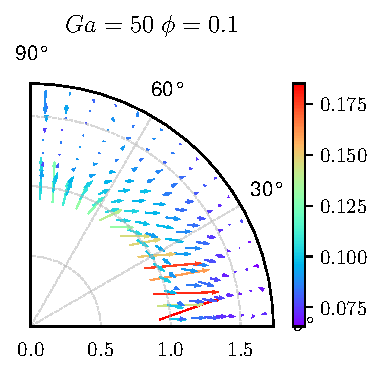
\includegraphics[width=0.9\textwidth]{image/HOMOGENEOUS/fDrop/F_mu_r_0_1_Ga_50_PHI_0_1.pdf}
%         \caption{Nearest relative averaged force fields, $\nstrelavg{\textbf{F}}(\textbf{r})$.}
%       \end{figure}
%       \column{0.5\textwidth}
%       \centering
%       \begin{figure}
%       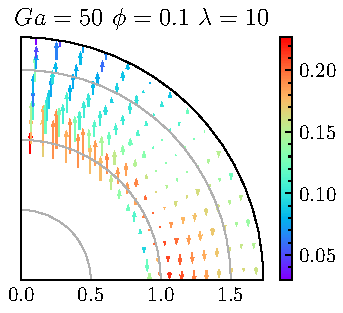
\includegraphics[width=0.9\textwidth]{image/HOMOGENEOUS/fDrop/U_mu_r_0_1_Ga_50_PHI_0_1.pdf}
%       \caption{Relative averaged velocity fields, $\nstavg{\textbf{w}}(\textbf{r})$.}
%     \end{figure}
%     \end{columns}
%   \end{columns}
%   \begin{itemize}
%     \item We notice that $F_c$ and $t_c$ are function of \textbf{r}, $\phi$, $Ga$, $\mu_r$ \ldots
%     \item Therefore,
%     $ h(t_c,F_n,\textbf{r})  \sim F_n(\textbf{r}) / t_c(\textbf{r}) D \sigma^{-1} \mu^{1/2}$
%   \end{itemize}
% \end{frame}

% \begin{frame}
%   \frametitle{Motion and coalesce of the nearest droplet}
% \centering
% \begin{tikzpicture}
%   \node (img) at (0,0) {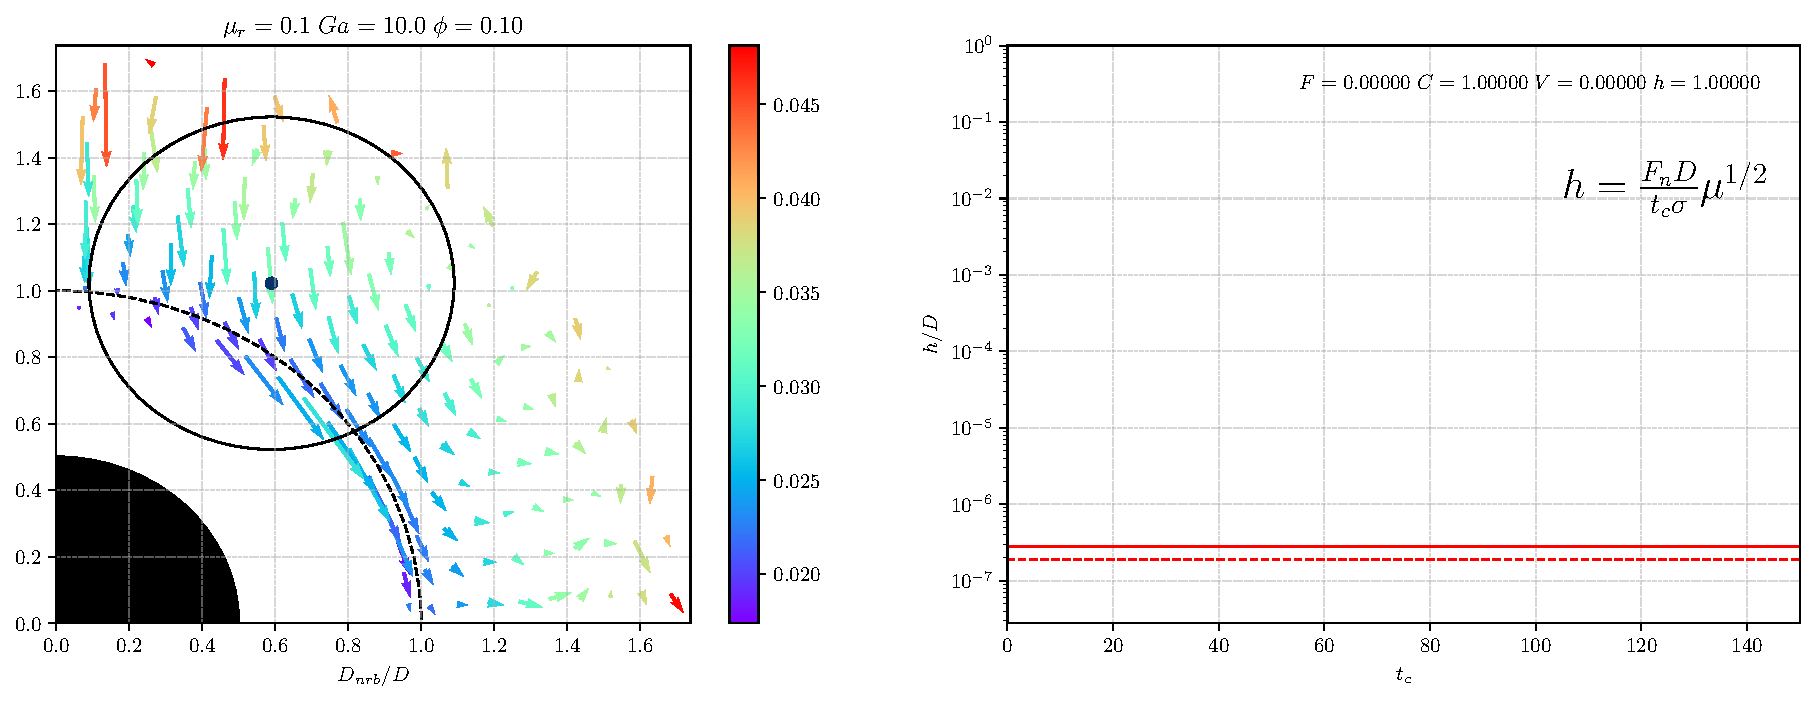
\includegraphics[width=\textwidth]{image/HOMOGENEOUS/anim/frame_1_0_1_Ga_10_PHI_0_1.pdf}};
%   \node (hc) at (1.4,-1.8) {\textcolor{red}{$h_c$}};
% \end{tikzpicture}
%   % \includegraphics[width=\textwidth]{../movies/P_PHI_1_Ga_75.gif}
  
%   $Ga = 10$ :
%   \href{file:///work/fintzin/BUBLLES_PROJECT/movies/First_anim.mp4}{\beamergotobutton{Play}}\\
%   $Ga = 25$ :
%   \href{file:///work/fintzin/BUBLLES_PROJECT/results/HOMOGENEOUS/Dim_3/N_5/PHI_0.1/rho_r_1.11/Bo_1/mu_r_0.1/Ga_25/animation_N1.mp4}{\beamergotobutton{Play}}\\
%   $Ga = 50$ :
%   \href{file:///work/fintzin/BUBLLES_PROJECT/results/HOMOGENEOUS/Dim_3/N_5/PHI_0.1/rho_r_1.11/Bo_1/mu_r_0.1/Ga_50/animation_N1.mp4}{\beamergotobutton{Play}}
% \end{frame}

% \begin{frame}
%   \frametitle{Motion and coalesce of the nearest droplets }
% \centering
%   \begin{tikzpicture}
%     \node (img) at (0,0) {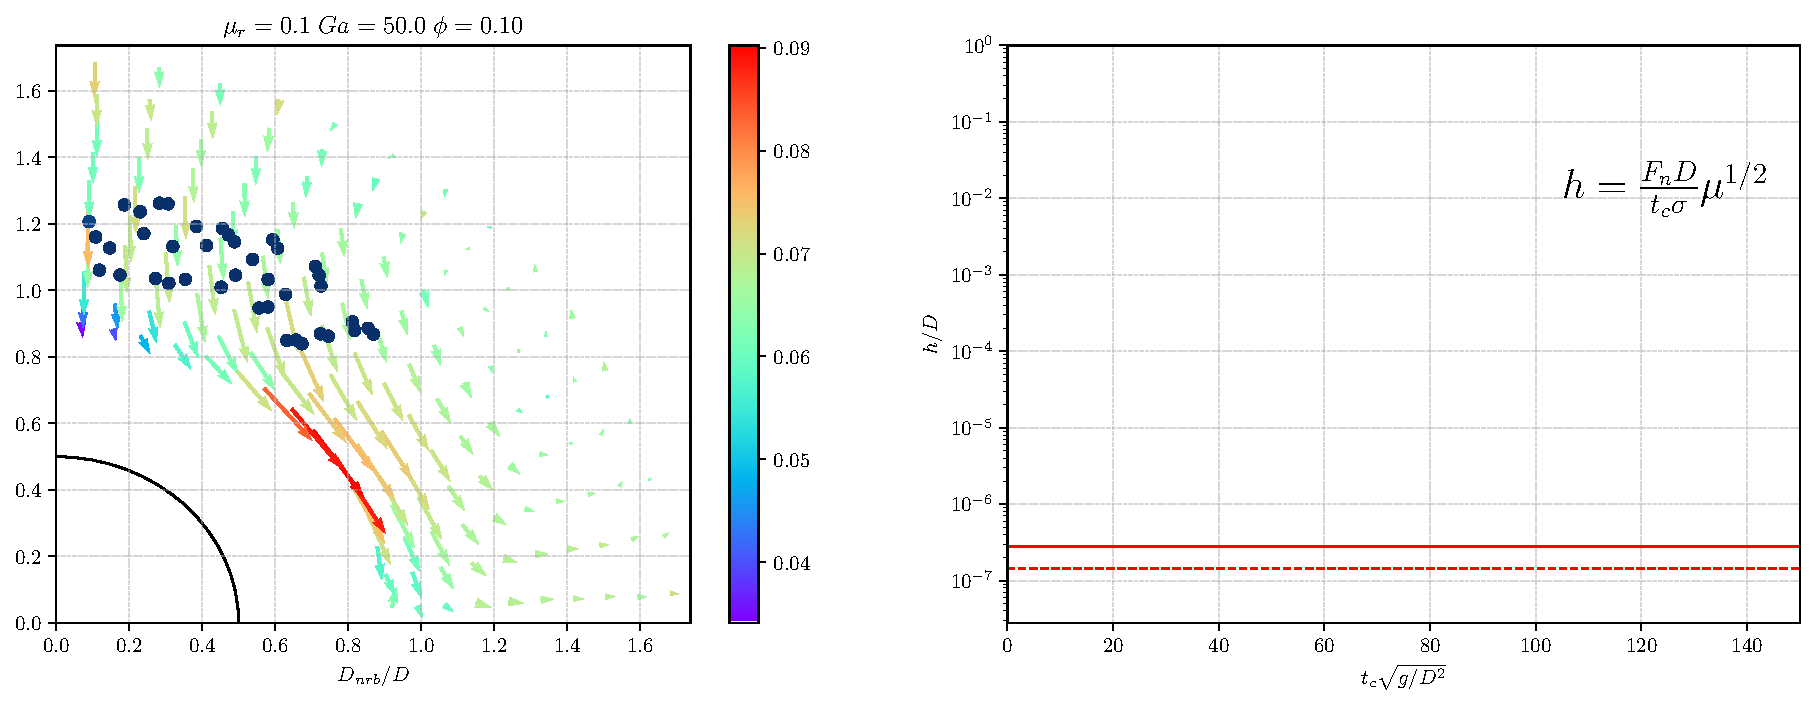
\includegraphics[width=\textwidth]{image/HOMOGENEOUS/anim/frame_1_N40_0_1_Ga_50_PHI_0_1.pdf}};
%     \node (hc) at (1.4,-1.8) {\textcolor{red}{$h_c$}};
%   \end{tikzpicture}
%   % \href{file:///work/fintzin/BUBLLES_PROJECT/results/HOMOGENEOUS/Dim_3/N_5/PHI_0.1/rho_r_1.11/Bo_1/mu_r_0.1/Ga_25/animation_N1.mp4}{\beamergotobutton{Play}}
  
%   \begin{columns}
%     \column{0.5\textwidth}
%     \centering
%     \begin{tabular}{|c|c|c|}\hline
%        &
%       $Ga = 10$ &
%       \href{file:///work/fintzin/BUBLLES_PROJECT/results/HOMOGENEOUS/Dim_3/N_5/PHI_0.1/rho_r_1.11/Bo_1/mu_r_0.1/Ga_10/animation.mp4}{\beamergotobutton{Play}}\\
%       $\phi = 0.1$&
%       $Ga = 25$ &
%       \href{file:///work/fintzin/BUBLLES_PROJECT/results/HOMOGENEOUS/Dim_3/N_5/PHI_0.1/rho_r_1.11/Bo_1/mu_r_0.1/Ga_25/animation.mp4}{\beamergotobutton{Play}}\\
%       &
%       $Ga = 50$ &
%       \href{file:///work/fintzin/BUBLLES_PROJECT/results/HOMOGENEOUS/Dim_3/N_5/PHI_0.1/rho_r_1.11/Bo_1/mu_r_0.1/Ga_50/animation.mp4}{\beamergotobutton{Play}}\\\hline
%     \end{tabular}
%     \column{0.5\textwidth}
%     \centering
%     \begin{tabular}{|c|c|c|}\hline
%       &
%      $Ga = 10$ &
%      \href{file:///work/fintzin/BUBLLES_PROJECT/results/HOMOGENEOUS/Dim_3/N_5/PHI_0.01/rho_r_1.11/Bo_1/mu_r_0.1/Ga_10/animation.mp4}{\beamergotobutton{Play}}\\
%      $\phi = 0.01$&
%      $Ga = 25$ &
%      \href{file:///work/fintzin/BUBLLES_PROJECT/results/HOMOGENEOUS/Dim_3/N_5/PHI_0.01/rho_r_1.11/Bo_1/mu_r_0.1/Ga_25/animation.mp4}{\beamergotobutton{Play}}\\
%      &
%      $Ga = 50$ &
%      \href{file:///work/fintzin/BUBLLES_PROJECT/results/HOMOGENEOUS/Dim_3/N_5/PHI_0.01/rho_r_1.11/Bo_1/mu_r_0.1/Ga_50/animation.mp4}{\beamergotobutton{Play}}\\\hline
%    \end{tabular}
%   \end{columns}
% \end{frame}

\section{Conclusion and perspectives}
\section*{}

% \begin{frame}
%   \frametitle{How to predict the rate of coalescing particles ?}
%   \underline{Assumed condition for the coalescence at a fixed time $t$ :}
%   \begin{itemize}
%     \item The interaction force must be low : $\textbf{f}_n \leq 0$ $\rightarrow$ $a > \tau$
%     \item Particles must remain in close contact : $\textbf{r} \leq D$. 
%   \end{itemize}
%   \vfill
%   Probable number of coalescing particles : 
%   \begin{align*}
%     C_{nst}(\textbf{x},t) 
%     &= \int_{|\textbf{r}|<D}\int_{a = \tau}^\infty P_{nst}(\textbf{x},\textbf{r},a,t)  d\textbf{r}da\\
%     &= \int_{|\textbf{r}|<D}\int_{a = \tau}^\infty P_{nst}(\textbf{r}|a>\tau,\textbf{x},t)\frac{e^{-a/\tau(\textbf{x})}}{\tau(\textbf{x})}  d\textbf{r}da\\
%     &= e^{-1}\int_{|\textbf{r}|<D} P_{nst}(\textbf{r}| a > \tau,\textbf{x},t)  \textbf{r}\\
%   \end{align*}
% \begin{itemize}
%   \item How to estimate $\int_{|\textbf{r}|<D} P_{nst}(\textbf{r}| a > \tau,t,\textbf{x})  d\textbf{r}$ ? 
% \end{itemize}
% \end{frame}

% \begin{frame}
%   \frametitle{First glimpse of coalescence kernel modeling}
%   Probable number of coalescing particles : 
%   \begin{equation*}
%     C_{nst}(\textbf{x},t,a) 
%     = e^{-1}\int_{|\textbf{r}|<D} P_{nst}(\textbf{r}| a > \tau,t,\textbf{x})d\textbf{r}
%   \end{equation*}
%   \begin{columns}
%     \column{0.3\textwidth}
%     \underline{Numerical results :}
%     \vfill
%     \begin{figure}
%       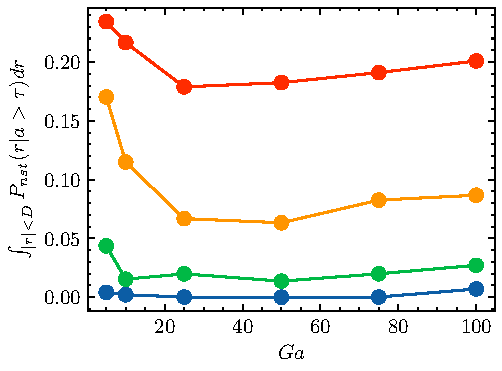
\includegraphics[height=0.8\textwidth]{image/HOMOGENEOUS/fPA/Proba.pdf}
%     \end{figure}
%     \column{0.6\textwidth}
%     \begin{itemize}
%       \item At low $Ga$ the forces of interaction is lower for close contact leading to a greater coalesence rate. 
%       \item At high $Ga$ the frequency of collision is higher leading to higher coalescence rate. 
%       \item The minimum of $C_{nst}$ arise at  $Ga =25$ because $\mathbb{R}(Ga=25)=\min(\mathbb{R})$
%     \end{itemize}
%   \end{columns}
% \end{frame}

\begin{frame}
  \frametitle{General remarks and conclusion}

  \begin{itemize}
    \item We used the nearest particle statistics to derive relative pair interactions equations. 
    \item We found out that relative velocity and forces are directly correlated to the relative position \textbf{r} and age of the interaction $a$, with $Ga$ and $\phi$. 
    \item The interaction relaxation time corresponds approximately to the mean age of interaction $\tau =\avg{a}$. 
  \end{itemize}
    \underline{Future projects : }  
    \begin{itemize}
      \item Studying the influence of poly-dispersity. 
      \item Deriving a rigorous formulation for the coalescence kernel which takes in account the physics of the film drainage problem. 
    \end{itemize}
\vfill    
% \vspace{1cm}
See my work : \url{http://basilisk.fr/sandbox/fintzin/Rising-Suspenion/}

\end{frame}

\begin{frame}
  \frametitle{Closure terms for the averaged Navier Stokes equation.}
\begin{columns}
  \begin{column}{0.5\textwidth}
    \begin{figure}
      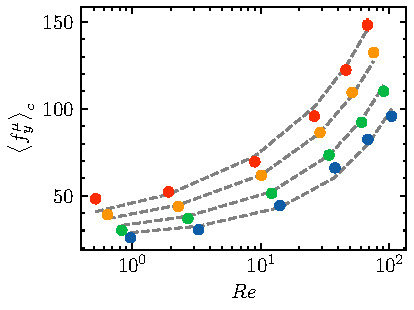
\includegraphics[width=0.7\textwidth]{image/HOMOGENEOUS/fCA/FH_mu_Re.pdf}
      \caption{Dimensionless drag force in terms $Re$ for $\phi = 0.01, 0.05, 0.1$ and $0.15$.}
    \end{figure}
    \begin{equation*}
      \frac{\avg{f}}{\mu UD} 
      = 1.18 e^{5.32\phi^{1/3}}  Re^{0.33}  + Re^{0.87} +24.12
    \end{equation*}
  \end{column}
  \begin{column}{0.5\textwidth}
    \begin{figure}[h!]
      \centering
      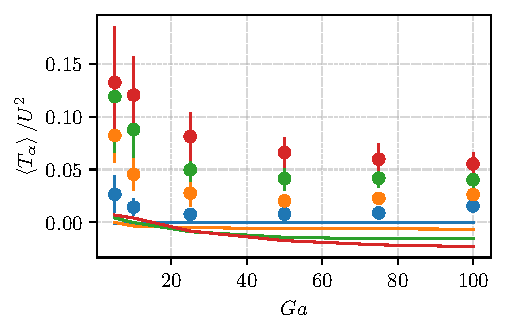
\includegraphics[width=0.7\textwidth]{image/HOMOGENEOUS/fPA/Talpha.pdf}
      \caption{Dimensionless granular temperature in terms of $Ga$ and $\phi$}
  \end{figure}
  	\begin{equation}
    \frac{\avg{\textbf{u}'\cdot \textbf{u}'}}{U^2}  
    \approx \frac{\phi}{Ga^2} 2.86 
    \label{eq:Talpha_scaling}
	\end{equation}
    % \begin{itemize}
    %   \item $U$ is the relative velocity between the continuous and dispersed phase.
    %   \item $Re$ is the \textit{Reynolds} number defined as, $Re = \rho D U / \mu$. 
    % \end{itemize}
  \end{column}
\end{columns}

\end{frame}

\begin{frame}[t]
  \frametitle{References}
  \bibliography{Bib/bib_bulles.bib}
\end{frame}

 
\backmatter

% \section{Evolution of interactions dynamics}

\section*{}

\begin{frame}
  \frametitle{Let study the interaction time between  a pair of the nearest particle}
    \begin{figure}
        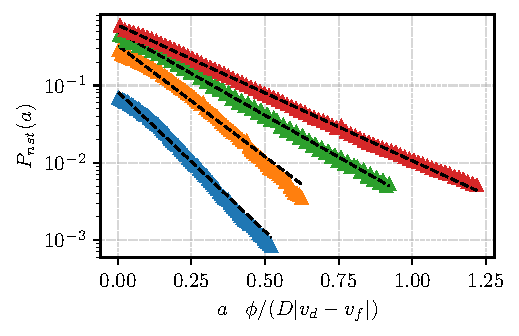
\includegraphics[height=0.23\textwidth]{image/HOMOGENEOUS/fDrop/P_a_Ga_25.pdf}
        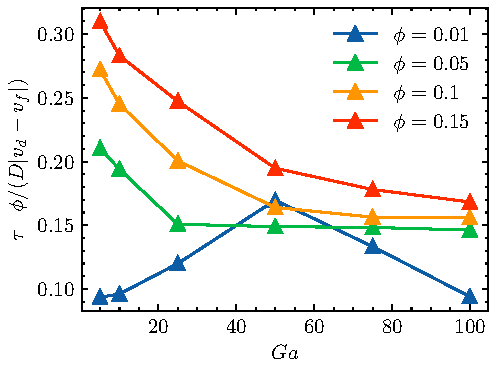
\includegraphics[height=0.23\textwidth]{image/HOMOGENEOUS/fPA/ageGa.pdf}
        \caption{ (left) PDF of the dimensionless age of interaction for fixed $Ga = 25$.
      (right) Mean time of interaction $\tau(\textbf{x})$.}
    \end{figure}
  \begin{equation*}
    P_{nst}(\textbf{x},a) 
    = \int P_{nst}(\textbf{x},\textbf{r},\textbf{w},a) d\textbf{w}d\textbf{r}
    \rightarrow\frac{e^{-a/\tau(\textbf{x})}}{\tau(\textbf{x})}
  \end{equation*}
\begin{itemize}
  \item $\tau(\textbf{x}) = \int a P_{nst}(\textbf{x},a) da$ is the mean interaction time at $\textbf{x}$. 
\end{itemize}
\end{frame}

\begin{frame}
  \frametitle{Position history of the interaction}
    \begin{figure}
        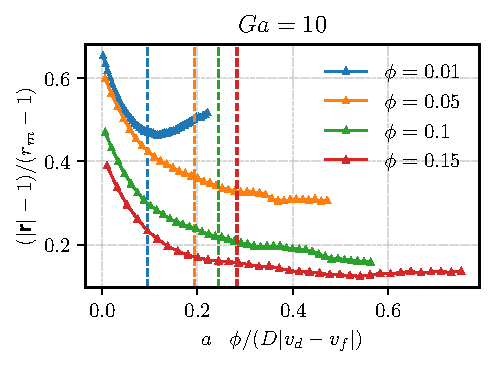
\includegraphics[height=0.23\textwidth]{image/HOMOGENEOUS/fDrop/r_a_Ga_10.pdf}
        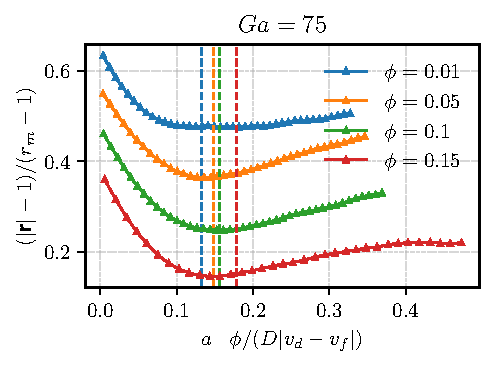
\includegraphics[height=0.23\textwidth]{image/HOMOGENEOUS/fDrop/r_a_Ga_75.pdf}
        \caption{ Conditional average $\nstavg{\textbf{r}}(a)$ on the age of the interaction} 
    \end{figure}
  \begin{equation*}
     \nstavg{\textbf{r}}(\textbf{x},a)
    = e^{a/\tau(\textbf{x})}\tau(\textbf{x})\int \textbf{r} P_{nst}(\textbf{x},\textbf{r},\textbf{w},a) d\textbf{w}d\textbf{r}
    % = \frac{e^{-a/\tau(\textbf{x})}}{\tau(\textbf{x})}
  \end{equation*}

\end{frame}


\begin{frame}
  \frametitle{Kinematic history of the interaction}
    \begin{figure}
        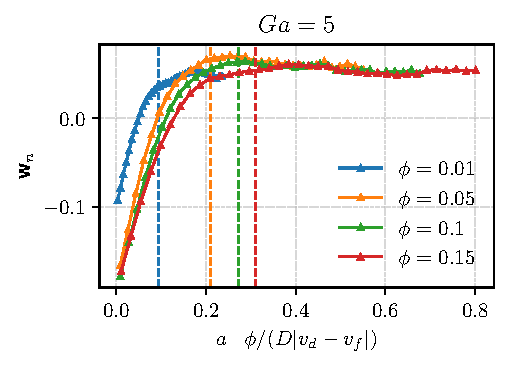
\includegraphics[height=0.24\textwidth]{image/HOMOGENEOUS/fDrop/ur_a_Ga_5.pdf}
        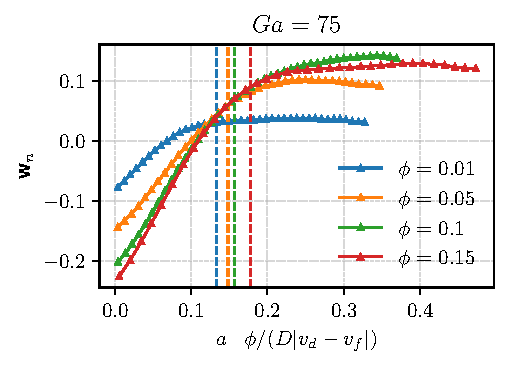
\includegraphics[height=0.24\textwidth]{image/HOMOGENEOUS/fDrop/ur_a_Ga_75.pdf}
        \caption{Conditional average of the normal relative velocity : $\nstavg{\textbf{w}_n}(a) = \nstavg{\textbf{w}}(a)\cdot \textbf{r}/|\textbf{r}|$ for $Ga = 5,100$ in terms of the dimensionless age $a$.
        (dashed lines) average time of interaction, $\tau(\textbf{x})$}. 
    \end{figure}
  \begin{equation*}
     \nstavg{\textbf{w}_n}(\textbf{x},a)
    = e^{a/\tau(\textbf{x})}\tau(\textbf{x})\int \textbf{w}\cdot(\textbf{r}/|\textbf{r}|) P_{nst}(\textbf{x},\textbf{r},\textbf{w},a) d\textbf{w}d\textbf{r}
    % = \frac{e^{-a/\tau(\textbf{x})}}{\tau(\textbf{x})}
  \end{equation*}

$\rightarrow$ $\tau(\textbf{x},a)$ correspond roughly to the relaxation time of $\nstavg{\textbf{w}_n}(\textbf{x},a)$
\end{frame}
\begin{frame}
  \frametitle{Dynamics history of the interaction}
    \begin{figure}
      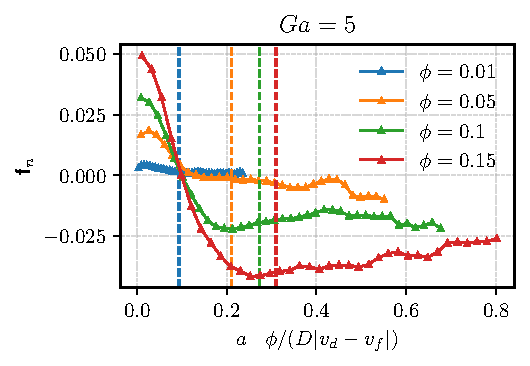
\includegraphics[height=0.24\textwidth]{image/HOMOGENEOUS/fDrop/f_a_Ga_5.pdf}
      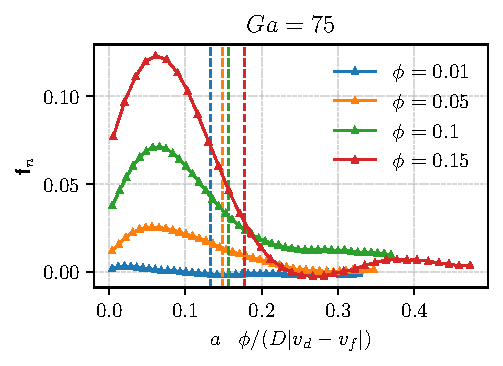
\includegraphics[height=0.24\textwidth]{image/HOMOGENEOUS/fDrop/f_a_Ga_75.pdf}
        \caption{Conditional average of the normal relative forces : $\nstavg{\textbf{f}_n}(a) = \nstavg{\textbf{f}}(a)\cdot \textbf{r}/|\textbf{r}|$ for $Ga = 5,10$ . 
        (dashed lines) avenged time of interaction, $\tau(\textbf{x})$}. 
    \end{figure}

\begin{itemize}
  \item $\tau(\textbf{x})$ correspond also to the relaxation of $\nstavg{\textbf{f}_n}(\textbf{x},a)$
  \item For $a > \tau(\textbf{x})$ we roughly have $\nstavg{\textbf{f}_n}(\textbf{x},a) \leq 0 $
\end{itemize}
$\rightarrow$After a time of interaction of $a \geq \tau$ the force is relatively low or attractive,  and the relative velocity is constant. 
\end{frame}


\begin{frame}
  \frametitle{Conditional average of the force on the velocity}
  \begin{figure}
    \centering
    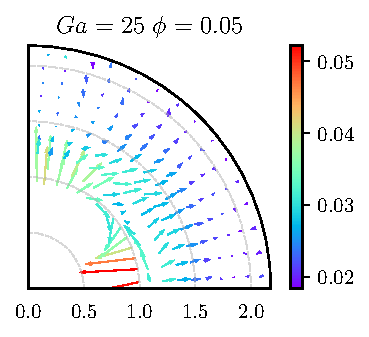
\includegraphics[width=0.33\textwidth]{image/HOMOGENEOUS/fDrop/F_mu_r_0_1_Ga_25_PHI_0_05.pdf}
    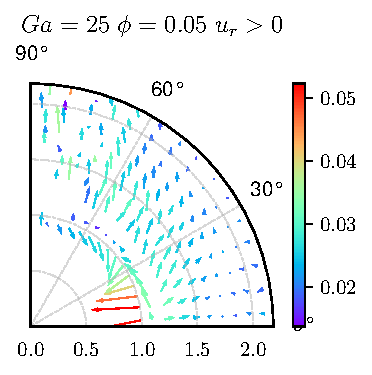
\includegraphics[width=0.33\textwidth]{image/HOMOGENEOUS/fDrop/Fpos_mu_r_0_1_Ga_25_PHI_0_05.pdf}
    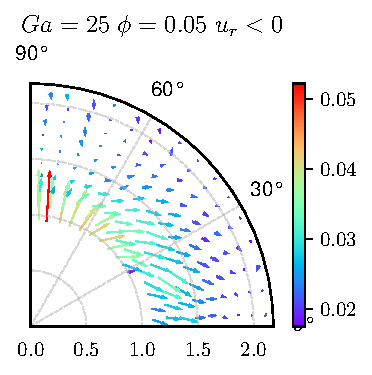
\includegraphics[width=0.33\textwidth]{image/HOMOGENEOUS/fDrop/Fneg_mu_r_0_1_Ga_25_PHI_0_05.pdf}
    \caption{Nearest averaged force fields, $\nstrelavg{\textbf{F}}(\textbf{r})$ for different $Ga$ and $\phi$. 
    Color map : Magnitude of the dimensionless force  $\nstrelavg{\textbf{F}} / (\Delta \rho V g)$.
    (middle) conditional average  $\nstrelavg{\textbf{F}| u_r > 0}(\textbf{r})$. 
    (right) conditional average  $\nstrelavg{\textbf{F}| u_r < 0}(\textbf{r})$ }
  \end{figure}
\end{frame}

\begin{frame}
  \frametitle{Conditional average of the force on the velocity}
  \begin{figure}
    \centering
    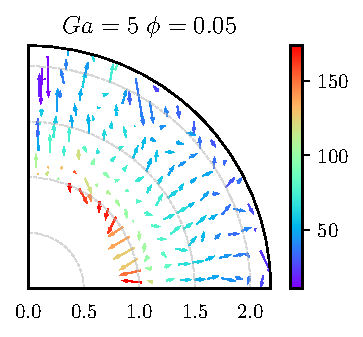
\includegraphics[width=0.33\textwidth]{image/HOMOGENEOUS/fDrop/F_mu_r_0_1_Ga_5_PHI_0_05.pdf}
    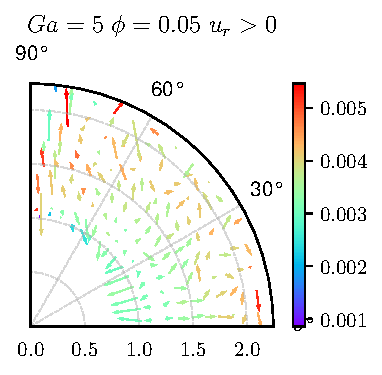
\includegraphics[width=0.33\textwidth]{image/HOMOGENEOUS/fDrop/Fpos_mu_r_0_1_Ga_5_PHI_0_05.pdf}
    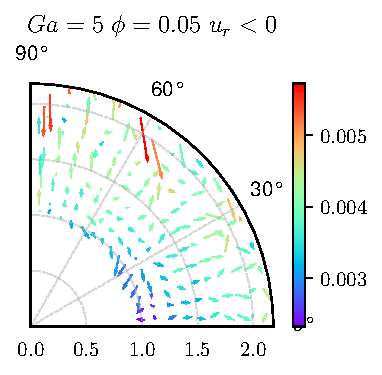
\includegraphics[width=0.33\textwidth]{image/HOMOGENEOUS/fDrop/Fneg_mu_r_0_1_Ga_5_PHI_0_05.pdf}
    \caption{Nearest averaged force fields, $\nstrelavg{\textbf{F}}(\textbf{r})$ for different $Ga$ and $\phi$. 
    Color map : Magnitude of the dimensionless force  $\nstrelavg{\textbf{F}} / (\Delta \rho V g)$.
    (middle) conditional average  $\nstrelavg{\textbf{F}| u_r > 0}(\textbf{r})$. 
    (right) conditional average  $\nstrelavg{\textbf{F}| u_r < 0}(\textbf{r})$ }
  \end{figure}
\end{frame}


\begin{frame}
  \frametitle{Article }
    \begin{itemize}
      \item Theoretical part with the transport equation of $P_{nst}$. 
      \begin{itemize}
        \item Based on the work of Zhang
        \item Define a coalescence kernel based on the age of interaction ?
      \end{itemize}
      \item Numerical method
      \begin{itemize}
        \item Ref to basilisk numerical method. 
        \item Need a validations 
        \begin{itemize}
          \item Same as the one in \citet{loisy2017buoyancy}
          \item A validations of the no.coalesce ??
        \end{itemize}
      \end{itemize}
      \item Presentation of the distribution $P_{nst} (\textbf{r},\textbf{w},a)$. 
      \item Presentation of the averaged moments of $\textbf{r}P_{nst}$ and their transport equations
      \item Physical interpretation 
      \item Conclusion 
      \begin{itemize}
        \item The moment average of $P_{nst}$ describe inter particle scale physics such as repulsion attraction among particle, it predicts cluster etc\ldots
        \item 
      \end{itemize}
    \end{itemize}

  

\end{frame}

\begin{frame}
  \frametitle{Others ideas :Create a restitution ratio of droplets}
  \begin{figure}
    \centering
    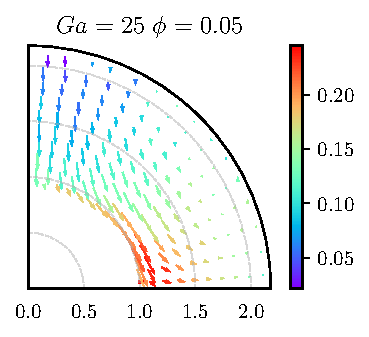
\includegraphics[width=0.27\textwidth]{image/HOMOGENEOUS/fDrop/U_mu_r_0_1_Ga_25_PHI_0_05.pdf}
    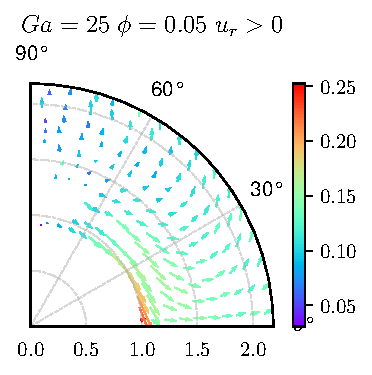
\includegraphics[width=0.27\textwidth]{image/HOMOGENEOUS/fDrop/Upos_mu_r_0_1_Ga_25_PHI_0_05.pdf}
    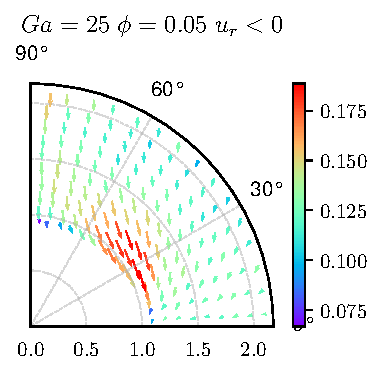
\includegraphics[width=0.27\textwidth]{image/HOMOGENEOUS/fDrop/Uneg_mu_r_0_1_Ga_25_PHI_0_05.pdf}
    \caption{Nearest averaged force fields, $\nstavg{\textbf{w}}(\textbf{r})$ for different $Ga$ and $\phi$. 
    Color map : Magnitude of the dimensionless force  $\nstavg{\textbf{w}} / (\Delta \rho V g)$.
    (middle) conditional average  $\nstrelavg{\textbf{u}| u_r > 0}(\textbf{r})$. 
    (right) conditional average  $\nstrelavg{\textbf{u}| u_r < 0}(\textbf{r})$ }
  \end{figure}
  \begin{equation}
    \text{Damping Ratio}
    \approx \frac{\avg{\frac{1}{2} \textbf{u} \cdot \textbf{u}| u_r > 0}}
    {\avg{\frac{1}{2}\textbf{u}\cdot \textbf{u}| u_r < 0}}
    = 0.12
  \end{equation}
Très interressant

\end{frame}

\begin{frame}
  \frametitle{Others ideas :}
  \begin{itemize}
    \item Create a coalescence kernel 
\end{itemize}
Définition of the PDF : 
  \begin{equation}
    P_{nst}(\textbf{x},\textbf{r},a)
    = \int \sum_i \sum_j 
    \delta_i(\textbf{x}-\textbf{x}_i)
    \delta_j(\textbf{x} + \textbf{r}-\textbf{x}_j)
    \delta(t - t-c -a)
    h_{ij}
    P(\mathscr{C})d\mathscr{C}
  \end{equation}
  Thus the collision kernel is : 
  \begin{equation}
    C_{nst}(\textbf{x},\textbf{r},a)
    = \int \sum_i \sum_j 
    \delta_i(\textbf{x}-\textbf{x}_i)
    \delta_j(\textbf{x} + \textbf{r}-\textbf{x}_j)
    \delta(t - t-c -a)
    h_{ij}
    P(\mathscr{C})d\mathscr{C}
  \end{equation}

\end{frame}

\begin{frame}
  \frametitle{Bilan Rénion :}
  \begin{itemize}
    \item Ne pas traiter de la coalesence dans le main papierIl faut absolument donner confiance dans les resultats 
    Montrer cliarement le but sans aller jusqu'au bout et ouvirir sur les perspective
    \item CCL : On a clarifié la physique entre pair 
    \item J ai quantifié des qte moyenne
    \item Validation de no-caloescen
    \begin{itemize}
      \item Faire une convergence en maillage pour voir si on dissipe 
      \item Comparer au cas de remonter de JL simu Plus expe
      \item décrire l'algo et regarder les papier sur les mousse, "foam or not to foam"
      \item décrire le fonctionnement du no coalescence
    \end{itemize}
    \item Ecrire un papier sur le fit du particule stress pour les gouttes et les bulles 
    \item coefficient de restitution, crée un context théorique prenant en compte ca pour les gouttes 
\end{itemize}
\end{frame}

\begin{frame}
  \frametitle{Nearest Eularian averaged velocity. }

\begin{equation*}
  \nstavg{\textbf{u}}(\textbf{x},\textbf{r})
  = \int 
  \textbf{u}(\textbf{x},t)
  \sum_{\alpha}
  \delta(\textbf{x}+\textbf{r}-\textbf{x}_\alpha(\CC,t))
  h_\alpha(\textbf{x})(\CC,t)
  d\CC
\end{equation*}
with $h_\alpha(\textbf{x}) = 1$ if and only if $\alpha$ is the nearest particle to the point $\textbf{x}$, $h_\alpha(\textbf{x}) = 0$ otherwise. 
  

\end{frame}


\begin{frame}
  \frametitle{Nearest Eularian averaged velocity in the drop referential. }
  \centering
  
  \begin{figure}
    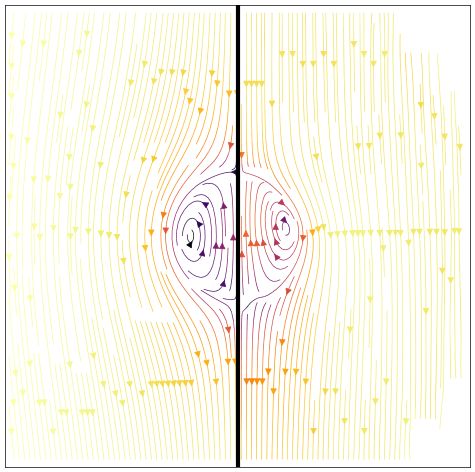
\includegraphics[height=0.4\textwidth]{image/Stream.png}
    \caption{(left)Stokes $\textbf{u} = (\textbf{g}+\textbf{d}\nabla^2) \mathcal{G}$; (right) DNS results $\nstavg{\textbf{u}}(\textbf{r})$ }
  \end{figure}
  \end{frame}
\begin{frame}
  \frametitle{Nearest Eularian averaged velocity in laboratory referential. }
  \centering
  
  \begin{figure}
    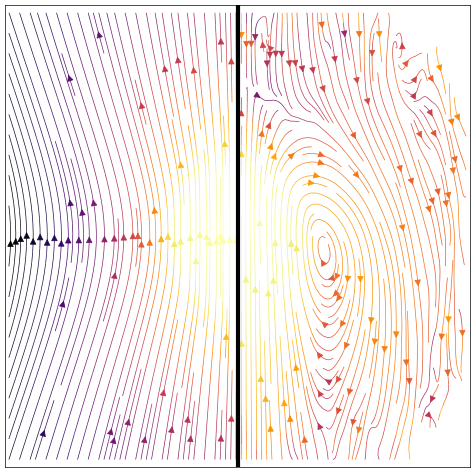
\includegraphics[height=0.4\textwidth]{image/Stream2.png}
    \caption{(left)Stokes $\textbf{u} = (\textbf{g}+\textbf{d}\nabla^2) \mathcal{G}$; (right) DNS results $\nstavg{\textbf{u}}(\textbf{r})$ }
  \end{figure}
  \end{frame}

\begin{frame}
  \frametitle{How to compute the fluid/particle fluctuation properly in DNS. }


We consider ergodicity at all time of the numerical experiment.
Thus, the statistical average of a local quantity $\textbf{u}^0$ is split into a spatial average $\Xavg{\textbf{u}^0}$ and a time average $\Tavg{\textbf{u}^0}$ such that $\textbf{u} = \avg{\textbf{u}^0} = \Xavg{\Tavg{\textbf{u}^0}}=\Tavg{\Xavg{\textbf{u}^0}}$.
Consequently, the ensemble average of a numerical field, $\textbf{u}^0$, is taken through space and time such that,
\begin{equation}
    \textbf{u}
    = \avg{\textbf{u}^0}
    = \Tavg{\Xavg{\textbf{u}^0}}
    = \frac{1}{t_{end}}\int_{0}^{t_{end}} 
    \Xavg{\textbf{u}^0}(t) dt
\end{equation}
where, 
\begin{equation}
    \Xavg{\textbf{u}^0}(t)
    = \frac{1}{L^3}\int 
    \textbf{u}^0(\textbf{x},t) d\textbf{x}
\end{equation}
  
\end{frame}
\begin{frame}
  \frametitle{How to compute the fluid/particle fluctuation properly in DNS. }
  First we expose our strategy to compute the continuous phase fluctuations. 
  It is computed as such, 
  \begin{equation}
      \phi_c \bm{\sigma}^{\text{Re}}_c /\rho_c
      = \avg{\chi_c \textbf{u}_c' \textbf{u}_c'}
      = \Tavg{\Xavg{\chi_c \textbf{u}_c' \textbf{u}_c'}}
      = \Tavg{\Xavg{\chi_c (\textbf{u}_c^0 -\textbf{u}_c ) (\textbf{u}_c^0 -\textbf{u}_c)}}
  \end{equation}
\begin{align*}
  \phi_c \bm{\sigma}^{\text{Re}}_c /\rho_c
    &= \Tavg{\Xavg{\chi_c \textbf{u}_c^0 \textbf{u}_c^0}}
    - \Tavg{\Xavg{\chi_c \textbf{u}_c^0 \textbf{u}_c}}
    - \Tavg{\Xavg{\chi_c \textbf{u}_c \textbf{u}_c^0}}
    + \Tavg{\Xavg{\chi_c \textbf{u}_c \textbf{u}_c}}\\
    &= \Tavg{\Xavg{\chi_c \textbf{u}_c^0 \textbf{u}_c^0}}
    -  \phi_c  \textbf{u}_c \textbf{u}_c 
\end{align*}
  
\end{frame}
\begin{frame}
  \frametitle{How to save our data. }
 Additionally, we can show
 \begin{align*}
  \phi_c \bm{\sigma}^{\text{Re}}_c /\rho_c
  &= 
  \underbrace{\Tavg{\Xavg{\chi_c (\textbf{u}_c^0 -\Xavg{\chi_c\textbf{u}_c^0} / \Xavg{\chi_c} ) (\textbf{u}_c^0 -\Xavg{\chi_c\textbf{u}_c^0} / \Xavg{\chi_c} )}}}_{\text{what we computed}}
  + \Tavg{\Xavg{\chi_c \textbf{u}_c^0}\Xavg{\chi_c\textbf{u}_c^0} / \Xavg{\chi_c}}
  -  \phi_c  \textbf{u}_c \textbf{u}_c 
\end{align*}
  
\end{frame}

\section*{On the capillary force }

\begin{frame}
  {The capilary force}
  2 = dispersed phase. 
  Force balance on the lfuid drop :
  \begin{equation*}
    \ddt \int_{V_\alpha} \rho_2 \textbf{u}^0_2 dV
    = 
    \int_{V_\alpha} \rho_2 \textbf{g} dV
    - \int_{S_\alpha} p_2 \textbf{n}_2 dS
    + \int_{S_\alpha} \mu_2 \textbf{S}_2 \cdot \textbf{n}_2 dS
  \end{equation*}

  interfaces Jump condition :
  \begin{align*}
    \Jump{\textbf{u}_k^0} = 0
    &&
    \Jump{-p_k^0 \textbf{I}+ \mu_k \textbf{S}_k^0} 
    =
    \sigma\textbf{n}\kappa
    \label{eq:surface_tension}
\end{align*}

\end{frame}

\begin{frame}
  {The capilary force}
  Let $S_c$ be the contact surface.
  \begin{equation*}
    \ddt \int_{V_\alpha} \rho_2 \textbf{u}^0_2 dV
    = 
    \int_{V_\alpha} \rho_2 \textbf{g} dV
    + \int_{S_\alpha} \mu_2 \textbf{S}_2 \cdot \textbf{n}_2 dS
    - \underbrace{\int_{S_c} p_2 \textbf{n}_2 dS}_\text{capilary force}
    - \int_{S_\alpha \backslash S_c} p_2 \textbf{n}_2 dS
  \end{equation*}

  interfaces Jump conditions integrated  on the contact surface :
  \begin{equation}
    \int_{S_c} \sigma\textbf{n}\kappa \; dS
    =
    \int_{S_c} \Jump{-p_k \textbf{I}+ \mu_k \textbf{S}_k} dS
\end{equation}

Thus the capillary force may be defined as : 
  \begin{equation}
    \int_{ S_c} p_1 \textbf{n}_2 dS
    =
    \int_{S_c} \sigma\textbf{n}\kappa \; dS
    + \int_{ S_c} p_2 \textbf{n}_2 dS
  \end{equation}
  In film drainage model it is assumed $\int_{S_c} \sigma\textbf{n}\kappa \; dS \approx 0 $ Thus, 
  \begin{equation*}
    \int_{ S_c} p_2 \textbf{n}_2 dS
    = \int_{ S} p_2 \textbf{n}_2 dS
    - \int_{ S \S_c} p_2 \textbf{n}_2 dS
  \end{equation*}

\end{frame}


\begin{frame}
  {First moment balance}
  \begin{equation}
    \ddt \mathcal{P}_\alpha
    = \int_{\Omega_\alpha} \left(
        \rho_2  \textbf{w}_2^0 \textbf{w}_2^0 
        - \bm{\sigma}_2^0
    \right) d\Omega
    + \int_{\Sigma_\alpha} \textbf{r}\bm{\sigma}_2^0\cdot\textbf{n}_2 d\Sigma
\end{equation}
interfaces Jump conditions integrated  on the contact surface :

\begin{equation}
  \int_{\Sigma_\alpha}
  \gamma (\textbf{I}-\textbf{nn})
  d\Sigma
  = 
  \int_{\Sigma_\alpha}\left(
    \Jump{\textbf{r}p_k}
    +
    \Jump{\textbf{r}\mu_k\textbf S_k }
    \right)
  d\Sigma
\end{equation}
Thus the previous balance in fact reads,
\begin{equation}
  \ddt \mathcal{P}_\alpha
  = \int_{\Omega_\alpha} \left(
      \rho_2  \textbf{w}_2^0 \textbf{w}_2^0 
      - \bm{\sigma}_2^0
  \right) d\Omega
  -\int_{\Sigma_\alpha}
  \gamma (\textbf{I}-\textbf{nn})
  d\Sigma 
  + \int_{\Sigma_\alpha} \textbf{r}\bm{\sigma}_1^0\cdot\textbf{n}_2 d\Sigma
\end{equation}
neglecting all inertial contribution : 
\begin{equation}
  \int_{\Sigma_\alpha}
  \gamma (\textbf{I}-\textbf{nn})
  d\Sigma 
  = \int_{\Omega_\alpha}
      p_2^0 \textbf{I}
   d\Omega
  + \int_{\Sigma_\alpha} p_1^0 \textbf{r}\textbf{n}_2 d\Sigma
\end{equation}



\end{frame}
\begin{frame}
  \frametitle{Trace First moment balance}
  \begin{align*}
    \ddt \int_{\Omega_\alpha}
    \textbf{r}\cdot\textbf{u}_2^0
    d\Omega
    &= \int_{\Omega_\alpha} 
    \rho_2  \textbf{w}_2^0 \cdot\textbf{w}_2^0 
    d\Omega
    - \int_{\Omega_\alpha} \left(
        - p_2^0
        + \mu_2\textbf{S}^0_2
    \right) d\Omega\\
    &-2\int_{\Sigma_\alpha}
    \gamma 
    d\Sigma 
    + \int_{\Sigma_\alpha} \textbf{r}\cdot \left(
      - p_1^0 \textbf{I}
      + \mu_1\textbf{S}^0_1
  \right)\cdot\textbf{n}_2 d\Sigma
  \end{align*}
  If we neglect all effect from inertia we obtain, 
  \begin{align*}
    2\int_{\Sigma_\alpha}
    \gamma 
    d\Sigma 
    =
    \int_{\Omega_\alpha} 
        p_2^0
     d\Omega
    - \int_{\Sigma_\alpha}
       p_1^0
      \textbf{r}\cdot \textbf{n}_2 d\Sigma
  \end{align*}
  

\end{frame}
\begin{frame}
  surface tension $\gamma$ is measured in
$N/m$, the unit of a spring stiffness: deforming a drop by a distance ε generates a restoring force
$\gamma$ $\epsilon$. 
A drop with mass $m$ impacting a repellent surface deforms but friction is clearly not dominant
since rebounds are observed. Hence, the elastic force $\gamma$ $\epsilon$ can be, to the first order, simply balanced
by the inertia $m\epsilon/\tau^2$ , denoting $\tau$ as the rebound time.
\end{frame}


\end{document}
